\section{Repeated measures by profile analysis}
\frame{\sectionpage}

\begin{frame}[fragile]{Repeated measures by profile analysis}

  \begin{itemize}
  \item More than one response {\em measurement} for each subject. Might be
    \begin{itemize}
    \item measurements of the same thing at different times
    \item measurements of different but related things
    \end{itemize}
  \item Generalization of matched pairs (``matched triples'', etc.).
  \item Variation: each subject does several different treatments at different times (called {\em crossover design}).
  \item Expect measurements on same subject to be correlated, so
    assumptions of independence will fail.
  \item Called {\em repeated measures}. Different approaches, but {\em
      profile analysis} uses \texttt{Manova} (set up right way).
  \item Another approach uses \emph{mixed models} (random effects).
  \end{itemize}
\end{frame}




\begin{frame}[fragile]{Example: histamine in dogs}
  
  \begin{itemize}
  \item 8 dogs take part in experiment.
  \item Dogs randomized to one of 2 different drugs.
  \item Response: log of blood concentration of histamine 0, 1, 3 and 5 minutes after taking drug. (Repeated measures.)
  \item Data in dogs.txt.
  \end{itemize}

\end{frame}

\begin{frame}[fragile]{Setting things up}


 
\begin{knitrout}
\definecolor{shadecolor}{rgb}{0.969, 0.969, 0.969}\color{fgcolor}\begin{kframe}
\begin{alltt}
\hlstd{dogs}\hlkwb{=}\hlkwd{read.table}\hlstd{(}\hlstr{"dogs.txt"}\hlstd{,}\hlkwc{header}\hlstd{=T)}
\hlstd{dogs}
\end{alltt}
\begin{verbatim}
##   dog         drug x   lh0   lh1   lh3   lh5
## 1   A     Morphine N -3.22 -1.61 -2.30 -2.53
## 2   B     Morphine N -3.91 -2.81 -3.91 -3.91
## 3   C     Morphine N -2.66  0.34 -0.73 -1.43
## 4   D     Morphine N -1.77 -0.56 -1.05 -1.43
## 5   E Trimethaphan N -3.51 -0.48 -1.17 -1.51
## 6   F Trimethaphan N -3.51  0.05 -0.31 -0.51
## 7   G Trimethaphan N -2.66 -0.19  0.07 -0.22
## 8   H Trimethaphan N -2.41  1.14  0.72  0.21
\end{verbatim}
\begin{alltt}
\hlstd{response}\hlkwb{=}\hlkwd{with}\hlstd{(dogs,}\hlkwd{cbind}\hlstd{(lh0,lh1,lh3,lh5))}
\hlstd{dogs.lm}\hlkwb{=}\hlkwd{lm}\hlstd{(response}\hlopt{~}\hlstd{drug,}\hlkwc{data}\hlstd{=dogs)}
\end{alltt}
\end{kframe}
\end{knitrout}
  
    
\end{frame}

\begin{frame}[fragile]{The repeated measures MANOVA}

Get list of response variable names; we call them \texttt{times}. Save
in data frame.

{\footnotesize
 
\begin{knitrout}
\definecolor{shadecolor}{rgb}{0.969, 0.969, 0.969}\color{fgcolor}\begin{kframe}
\begin{alltt}
\hlstd{times}\hlkwb{=}\hlkwd{colnames}\hlstd{(response)}
\hlstd{times.df}\hlkwb{=}\hlkwd{data.frame}\hlstd{(times)}
\hlstd{dogs.manova}\hlkwb{=}\hlstd{car}\hlopt{::}\hlkwd{Manova}\hlstd{(dogs.lm,}\hlkwc{idata}\hlstd{=times.df,}
     \hlkwc{idesign}\hlstd{=}\hlopt{~}\hlstd{times)}
\hlstd{dogs.manova}
\end{alltt}
\begin{verbatim}
## 
## Type II Repeated Measures MANOVA Tests: Pillai test statistic
##             Df test stat approx F num Df den Df   Pr(>F)   
## (Intercept)  1   0.76347  19.3664      1      6 0.004565 **
## drug         1   0.34263   3.1272      1      6 0.127406   
## times        1   0.94988  25.2690      3      4 0.004631 **
## drug:times   1   0.89476  11.3362      3      4 0.020023 * 
## ---
## Signif. codes:  0 '***' 0.001 '**' 0.01 '*' 0.05 '.' 0.1 ' ' 1
\end{verbatim}
\end{kframe}
\end{knitrout}
}

Interaction significant. Pattern of response over time different
for the two drugs.
\end{frame}

\begin{frame}[fragile]{Wide and long format}

  \begin{itemize}
  \item Want to investigate interaction.
  \item But data frame has several observations per line (``wide format''):
 
\begin{knitrout}
\definecolor{shadecolor}{rgb}{0.969, 0.969, 0.969}\color{fgcolor}\begin{kframe}
\begin{alltt}
\hlkwd{head}\hlstd{(dogs,}\hlkwc{n}\hlstd{=}\hlnum{5}\hlstd{)}
\end{alltt}
\begin{verbatim}
##   dog         drug x   lh0   lh1   lh3   lh5
## 1   A     Morphine N -3.22 -1.61 -2.30 -2.53
## 2   B     Morphine N -3.91 -2.81 -3.91 -3.91
## 3   C     Morphine N -2.66  0.34 -0.73 -1.43
## 4   D     Morphine N -1.77 -0.56 -1.05 -1.43
## 5   E Trimethaphan N -3.51 -0.48 -1.17 -1.51
\end{verbatim}
\end{kframe}
\end{knitrout}
    
  \item Plotting works with data in ``long format'':
    one response per line.
  \item The responses are log-histamine at different times, labelled
    \texttt{lh}-something. Call them all \texttt{lh} and put them in
    one column, with the time they belong to labelled.
  \end{itemize}
  
\end{frame}


\begin{frame}[fragile]{Running \texttt{gather}, try 1}
  
  \texttt{gather} needs: name for thing that makes columns different
  (time), name for thing that makes columns same (they are all values
  of log-histamine), and columns to combine:

  {\small
\begin{knitrout}
\definecolor{shadecolor}{rgb}{0.969, 0.969, 0.969}\color{fgcolor}\begin{kframe}
\begin{alltt}
\hlstd{dogs} \hlopt \hlkwd{gather}\hlstd{(time,lh,lh0}\hlopt{:}\hlstd{lh5)} \hlopt \hlkwd{head}\hlstd{(}\hlnum{12}\hlstd{)}
\end{alltt}
\begin{verbatim}
##    dog         drug x time    lh
## 1    A     Morphine N  lh0 -3.22
## 2    B     Morphine N  lh0 -3.91
## 3    C     Morphine N  lh0 -2.66
## 4    D     Morphine N  lh0 -1.77
## 5    E Trimethaphan N  lh0 -3.51
## 6    F Trimethaphan N  lh0 -3.51
## 7    G Trimethaphan N  lh0 -2.66
## 8    H Trimethaphan N  lh0 -2.41
## 9    A     Morphine N  lh1 -1.61
## 10   B     Morphine N  lh1 -2.81
## 11   C     Morphine N  lh1  0.34
## 12   D     Morphine N  lh1 -0.56
\end{verbatim}
\end{kframe}
\end{knitrout}
}
  
\end{frame}

\begin{frame}[fragile]{Splitting off the times}
  
Not quite right: for the times, we want just the numbers, not the
letters \texttt{lh} every time. Want new variable
containing just number in \texttt{time}:
\texttt{parse\_number}. (Actually  lives in \texttt{readr}, so
\texttt{library(tidyverse)} right way to go.)

{\small
\begin{knitrout}
\definecolor{shadecolor}{rgb}{0.969, 0.969, 0.969}\color{fgcolor}\begin{kframe}
\begin{alltt}
\hlstd{dogs} \hlopt \hlkwd{gather}\hlstd{(timex,lh,lh0}\hlopt{:}\hlstd{lh5)} \hlopt
    \hlkwd{mutate}\hlstd{(}\hlkwc{time}\hlstd{=}\hlkwd{parse_number}\hlstd{(timex))} \hlopt \hlkwd{head}\hlstd{(}\hlnum{10}\hlstd{)}
\end{alltt}
\begin{verbatim}
##    dog         drug x timex    lh time
## 1    A     Morphine N   lh0 -3.22    0
## 2    B     Morphine N   lh0 -3.91    0
## 3    C     Morphine N   lh0 -2.66    0
## 4    D     Morphine N   lh0 -1.77    0
## 5    E Trimethaphan N   lh0 -3.51    0
## 6    F Trimethaphan N   lh0 -3.51    0
## 7    G Trimethaphan N   lh0 -2.66    0
## 8    H Trimethaphan N   lh0 -2.41    0
## 9    A     Morphine N   lh1 -1.61    1
## 10   B     Morphine N   lh1 -2.81    1
\end{verbatim}
\end{kframe}
\end{knitrout}
}

\end{frame}

\begin{frame}[fragile]{What I did differently}
  
  \begin{itemize}
  \item I realized that \texttt{gather} was going to produce something
    like \texttt{lh1}, which I needed to do something further with, so
    this time I gave it a temporary name \texttt{timex}.
  \item This enabled me to use the name \texttt{time} for the actual
    numeric time.
  \item This works now, so next save into a new data frame \texttt{dogs.long}.
  \end{itemize}
  
\end{frame}

\begin{frame}[fragile]{Saving the chained results}
  

\begin{knitrout}
\definecolor{shadecolor}{rgb}{0.969, 0.969, 0.969}\color{fgcolor}\begin{kframe}
\begin{alltt}
\hlstd{dogs} \hlopt \hlkwd{gather}\hlstd{(timex,lh,lh0}\hlopt{:}\hlstd{lh5)} \hlopt
    \hlkwd{mutate}\hlstd{(}\hlkwc{time}\hlstd{=}\hlkwd{parse_number}\hlstd{(timex))}  \hlkwb{->} \hlstd{dogs.long}
\end{alltt}
\end{kframe}
\end{knitrout}

This says:

\begin{itemize}
\item Take data frame dogs, and then:
\item Combine the columns \texttt{lh0} through \texttt{lh5} into one
  column called \texttt{lh}, with the column that each \texttt{lh}
  value originally came from labelled by \texttt{timex}, and then:
\item Pull out numeric values in \texttt{timex}, saving in \texttt{time} and then:
\item save the result in a data frame \texttt{dogs.long}.
\end{itemize}
  
\end{frame}

%
%\begin{frame}[fragile]{\texttt{reshape}}
%
%  \begin{itemize}
%  \item Converts between wide and long format.
%  \item Need to tell R what our repeated-measures responses are.
%  \item Convenient variable naming: all responses are \texttt{lh}
%    followed by a number representing time.
%  \item Like this:
%  \end{itemize}
%
% 
%<<>>=
%detach(dogs)
%d2=reshape(dogs,varying=3:6,sep="",
%    direction="long")
%@ %def 
%
%\end{frame}
%
%\begin{frame}[fragile]{Long data frame, top 12 lines}
%
% 
%<<>>=
%head(d2,n=12)
%@ %def 
%  
%
%\texttt{id}  labels dog, \texttt{time} labels time. Perfect for
%interaction plot.
%  
%\end{frame}
%

\begin{frame}[fragile]{Interaction plot}
  
\begin{knitrout}
\definecolor{shadecolor}{rgb}{0.969, 0.969, 0.969}\color{fgcolor}\begin{kframe}
\begin{alltt}
\hlkwd{ggplot}\hlstd{(dogs.long,}\hlkwd{aes}\hlstd{(}\hlkwc{x}\hlstd{=time,}\hlkwc{y}\hlstd{=lh,}\hlkwc{colour}\hlstd{=drug,}\hlkwc{group}\hlstd{=drug))}\hlopt{+}
  \hlkwd{stat_summary}\hlstd{(}\hlkwc{fun.y}\hlstd{=mean,}\hlkwc{geom}\hlstd{=}\hlstr{"point"}\hlstd{)}\hlopt{+}
  \hlkwd{stat_summary}\hlstd{(}\hlkwc{fun.y}\hlstd{=mean,}\hlkwc{geom}\hlstd{=}\hlstr{"line"}\hlstd{)}
\end{alltt}
\end{kframe}
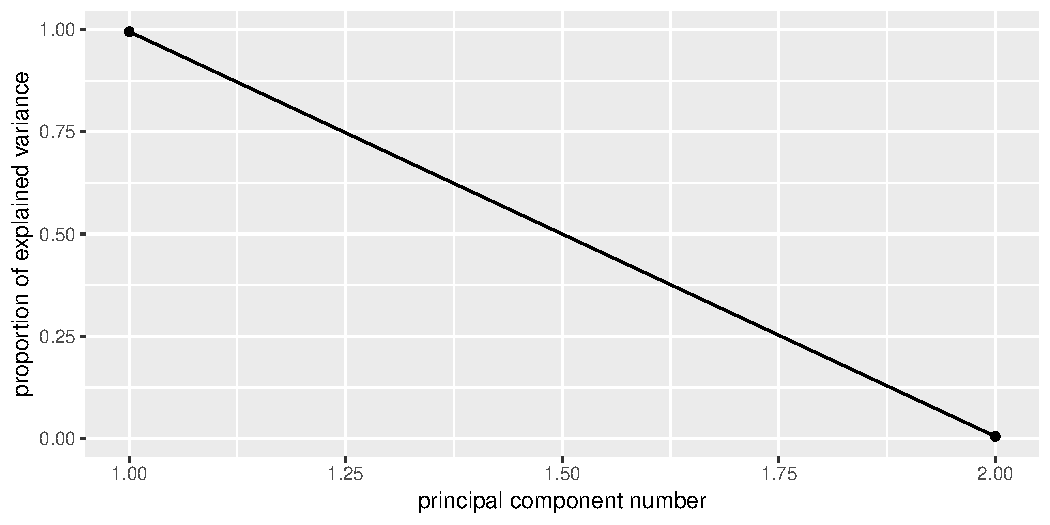
\includegraphics[width=\maxwidth]{figure/unnamed-chunk-8-1} 

\end{knitrout}
  
\end{frame}


\begin{frame}[fragile]{Comments}
  

\begin{itemize}
\item Plot mean \texttt{lh} value at each time, joining points on same
  drug by lines.
\item drugs same at time 0
\item after that, Trimethaphan higher than Morphine.
\item Effect of drug not consistent over time: significant interaction.
\end{itemize}

\end{frame}



\begin{frame}[fragile]{Take out time zero}

  \begin{itemize}
  \item Lines on interaction plot would then be parallel, and so interaction should
no longer be significant.
\item Go back to original ``wide'' \texttt{dogs} data frame.
  \end{itemize}
  

 
\begin{knitrout}
\definecolor{shadecolor}{rgb}{0.969, 0.969, 0.969}\color{fgcolor}\begin{kframe}
\begin{alltt}
\hlstd{response}\hlkwb{=}\hlkwd{with}\hlstd{(dogs,}\hlkwd{cbind}\hlstd{(lh1,lh3,lh5))} \hlcom{# excluding time zero}
\hlstd{dogs.lm}\hlkwb{=}\hlkwd{lm}\hlstd{(response}\hlopt{~}\hlstd{drug,}\hlkwc{data}\hlstd{=dogs)}
\hlstd{times}\hlkwb{=}\hlkwd{colnames}\hlstd{(response)}
\hlstd{times.df}\hlkwb{=}\hlkwd{data.frame}\hlstd{(times)}
\hlstd{dogs.manova}\hlkwb{=}\hlstd{car}\hlopt{::}\hlkwd{Manova}\hlstd{(dogs.lm,}\hlkwc{idata}\hlstd{=times.df,}
                   \hlkwc{idesign}\hlstd{=}\hlopt{~}\hlstd{times)}
\end{alltt}
\end{kframe}
\end{knitrout}


\end{frame}

\begin{frame}[fragile]{Results and comments}

{\small
 
\begin{knitrout}
\definecolor{shadecolor}{rgb}{0.969, 0.969, 0.969}\color{fgcolor}\begin{kframe}
\begin{alltt}
\hlstd{dogs.manova}
\end{alltt}
\begin{verbatim}
## 
## Type II Repeated Measures MANOVA Tests: Pillai test statistic
##             Df test stat approx F num Df den Df   Pr(>F)   
## (Intercept)  1   0.54582   7.2106      1      6 0.036281 * 
## drug         1   0.44551   4.8207      1      6 0.070527 . 
## times        1   0.85429  14.6569      2      5 0.008105 **
## drug:times   1   0.43553   1.9289      2      5 0.239390   
## ---
## Signif. codes:  0 '***' 0.001 '**' 0.01 '*' 0.05 '.' 0.1 ' ' 1
\end{verbatim}
\end{kframe}
\end{knitrout}
}

\begin{itemize}
\item Correct: interaction no longer significant.
\item Significant effect of time.
\item Drug effect not quite significant (some variety among dogs
  within drug).
\end{itemize}
  
\end{frame}

\begin{frame}[fragile]{Is the non-significant drug effect reasonable?}
  
  \begin{itemize}
  \item Plot \emph{actual data}: \texttt{lh} against \texttt{days},
    labelling observations by drug: ``spaghetti plot''.
  \item Uses long data frame (confusing, yes I know):
 

\item Plot (time,lh) points coloured  by drug
\item and connecting measurements for each \emph{dog} by lines.

  
\item This time, we want \texttt{group=dog} (want the measurements for each
\emph{dog} joined by lines), but \texttt{colour=drug}:
  
\begin{knitrout}
\definecolor{shadecolor}{rgb}{0.969, 0.969, 0.969}\color{fgcolor}\begin{kframe}
\begin{alltt}
\hlstd{g}\hlkwb{=}\hlkwd{ggplot}\hlstd{(dogs.long,}\hlkwd{aes}\hlstd{(}\hlkwc{x}\hlstd{=time,}\hlkwc{y}\hlstd{=lh,}
    \hlkwc{colour}\hlstd{=drug,}\hlkwc{group}\hlstd{=dog))} \hlopt{+}
  \hlkwd{geom_point}\hlstd{()}\hlopt{+}\hlkwd{geom_line}\hlstd{()}
\end{alltt}
\end{kframe}
\end{knitrout}
\end{itemize}
  
\end{frame}

\begin{frame}[fragile]{The spaghetti plot}
  
\begin{knitrout}
\definecolor{shadecolor}{rgb}{0.969, 0.969, 0.969}\color{fgcolor}\begin{kframe}
\begin{alltt}
\hlstd{g}
\end{alltt}
\end{kframe}
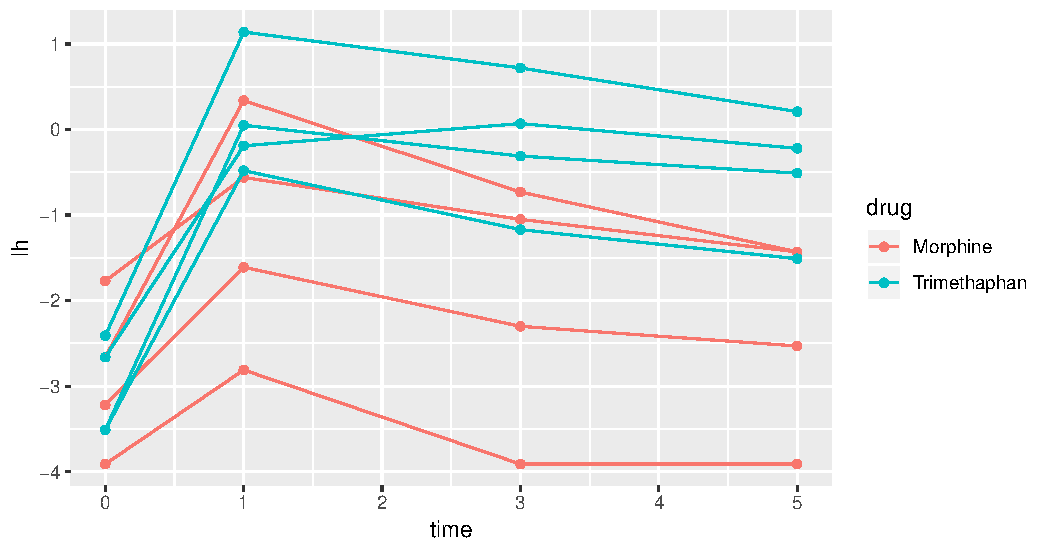
\includegraphics[width=\maxwidth]{figure/hoverla-1} 

\end{knitrout}
  
\end{frame}

\begin{frame}[fragile]{Comments}
  
  \begin{itemize}
  \item For each dog over time, there is a strong increase and gradual
    decrease in log-histamine. This
    explains the significant time effect.
  \item The pattern is more or less the same for each dog, regardless
    of drug. This explains the non-significant interaction.
  \item Most of the trimethaphan dogs (blue) have higher log-histamine
    throughout (time 1 and after), and some of the morphine dogs have
    lower.
  \item \emph{But} two of the morphine dogs have log-histamine
    profiles like the trimethaphan dogs. This ambiguity is probably
    why the \texttt{drug} effect is not quite significant.
  \end{itemize}
  
\end{frame}

 
\begin{frame}[fragile]{The exercise data}
  
  \begin{itemize}
  \item 30 people took part in an exercise study.
  \item Each subject was
    randomly assigned to one of two diets (``low fat'' or ``non-low
    fat'') and to one of three exercise programs (``at rest'',
    ``walking'', ``running'').
  \item There are $2\times3 = 6$ experimental treatments, and thus
    each one is replicated $30/6=5$ times.
  \item Nothing unusual so far.
  \item However, each subject had their pulse rate measured at three
    different times (1, 15 and 30 minutes after starting their
    exercise), so have repeated measures.
  \end{itemize}
  
\end{frame}

\begin{frame}[fragile]{The data}
  
\begin{knitrout}
\definecolor{shadecolor}{rgb}{0.969, 0.969, 0.969}\color{fgcolor}\begin{kframe}
\begin{alltt}
\hlstd{exercise.long}\hlkwb{=}\hlkwd{read.table}\hlstd{(}\hlstr{"exercise.txt"}\hlstd{,}\hlkwc{header}\hlstd{=T)}
\hlkwd{head}\hlstd{(exercise.long,}\hlnum{8}\hlstd{)}
\end{alltt}
\begin{verbatim}
##   id      diet exertype pulse  time
## 1  1 nonlowfat   atrest    85 min01
## 2  1 nonlowfat   atrest    85 min15
## 3  1 nonlowfat   atrest    88 min30
## 4  2 nonlowfat   atrest    90 min01
## 5  2 nonlowfat   atrest    92 min15
## 6  2 nonlowfat   atrest    93 min30
## 7  3 nonlowfat   atrest    97 min01
## 8  3 nonlowfat   atrest    97 min15
\end{verbatim}
\end{kframe}
\end{knitrout}

\begin{itemize}
\item This is ``long format'', which is usually what we want.
\item But for repeated measures analysis, we want \emph{wide} format!
\item \texttt{tidyr}: ``undo'' gather: \texttt{spread}.
\end{itemize}
  
\end{frame}

\begin{frame}[fragile]{Making wide format}
  
  \begin{itemize}
  \item Spread needs three things: a data frame, a column that is
    going to be split, and the column to make the values out of:
    
\begin{knitrout}
\definecolor{shadecolor}{rgb}{0.969, 0.969, 0.969}\color{fgcolor}\begin{kframe}
\begin{alltt}
\hlkwd{library}\hlstd{(tidyr)}
\hlstd{exercise.wide}\hlkwb{=}\hlkwd{spread}\hlstd{(exercise.long,time,pulse)}
\hlkwd{head}\hlstd{(exercise.wide)}
\end{alltt}
\begin{verbatim}
##   id      diet exertype min01 min15 min30
## 1  1 nonlowfat   atrest    85    85    88
## 2  2 nonlowfat   atrest    90    92    93
## 3  3 nonlowfat   atrest    97    97    94
## 4  4 nonlowfat   atrest    80    82    83
## 5  5 nonlowfat   atrest    91    92    91
## 6  6    lowfat   atrest    83    83    84
\end{verbatim}
\end{kframe}
\end{knitrout}
\item See how we would normally \texttt{gather} \texttt{min01, min15,
    min30} into one column called \texttt{pulse} labelled by the
  number of minutes? But \texttt{Manova} needs it the other way.
  \end{itemize}
  
\end{frame}

\begin{frame}[fragile]{Setting up the repeated-measures analysis}
  
  \begin{itemize}
  \item Make a response variable consisting of \texttt{min01, min15, min30}:
\begin{knitrout}
\definecolor{shadecolor}{rgb}{0.969, 0.969, 0.969}\color{fgcolor}\begin{kframe}
\begin{alltt}
\hlstd{response}\hlkwb{=}\hlkwd{with}\hlstd{(exercise.wide,}\hlkwd{cbind}\hlstd{(min01, min15, min30))}
\end{alltt}
\end{kframe}
\end{knitrout}
\item Predict that from \texttt{diet} and \texttt{exertype} and
  interaction using \texttt{lm}:
\begin{knitrout}
\definecolor{shadecolor}{rgb}{0.969, 0.969, 0.969}\color{fgcolor}\begin{kframe}
\begin{alltt}
\hlstd{exercise.1}\hlkwb{=}\hlkwd{lm}\hlstd{(response}\hlopt{~}\hlstd{diet}\hlopt{*}\hlstd{exertype,}
  \hlkwc{data}\hlstd{=exercise.wide)}
\end{alltt}
\end{kframe}
\end{knitrout}

\item Run this through \texttt{Manova}:
\begin{knitrout}
\definecolor{shadecolor}{rgb}{0.969, 0.969, 0.969}\color{fgcolor}\begin{kframe}
\begin{alltt}
\hlstd{times}\hlkwb{=}\hlkwd{colnames}\hlstd{(response)}
\hlstd{times.df}\hlkwb{=}\hlkwd{data.frame}\hlstd{(times)}
\hlstd{exercise.2}\hlkwb{=}\hlstd{car}\hlopt{::}\hlkwd{Manova}\hlstd{(exercise.1,}\hlkwc{idata}\hlstd{=times.df,}
                  \hlkwc{idesign}\hlstd{=}\hlopt{~}\hlstd{times)}
\end{alltt}
\end{kframe}
\end{knitrout}
  \end{itemize}
  
\end{frame}

\begin{frame}[fragile]{Results}
  
  
  \begin{scriptsize}
\begin{knitrout}
\definecolor{shadecolor}{rgb}{0.969, 0.969, 0.969}\color{fgcolor}\begin{kframe}
\begin{alltt}
\hlstd{exercise.2}
\end{alltt}
\begin{verbatim}
## 
## Type II Repeated Measures MANOVA Tests: Pillai test statistic
##                     Df test stat approx F num Df den Df    Pr(>F)    
## (Intercept)          1   0.99767  10296.7      1     24 < 2.2e-16 ***
## diet                 1   0.37701     14.5      1     24 0.0008483 ***
## exertype             2   0.79972     47.9      2     24 4.166e-09 ***
## diet:exertype        2   0.28120      4.7      2     24 0.0190230 *  
## times                1   0.78182     41.2      2     23 2.491e-08 ***
## diet:times           1   0.25153      3.9      2     23 0.0357258 *  
## exertype:times       2   0.83557      8.6      4     48 2.538e-05 ***
## diet:exertype:times  2   0.51750      4.2      4     48 0.0054586 ** 
## ---
## Signif. codes:  0 '***' 0.001 '**' 0.01 '*' 0.05 '.' 0.1 ' ' 1
\end{verbatim}
\end{kframe}
\end{knitrout}
  \end{scriptsize}

\begin{itemize}
\item Three-way interaction significant, so cannot remove anything.
\item Pulse rate depends on diet and exercise type \emph{combination},
  and \emph{that} is different for each time.
\end{itemize}
  
\end{frame}

\begin{frame}[fragile]{Making some graphs}
  
  \begin{itemize}
  \item Three-way  interactions are difficult to understand. To make
    an attempt, look at some graphs.
  \item Plot time trace of pulse rates for each individual, joined by
    lines, and make \emph{separate} plots for each
    \texttt{diet-exertype} combo.
  \item \texttt{ggplot} again. Using \emph{long} data frame:

\begin{knitrout}
\definecolor{shadecolor}{rgb}{0.969, 0.969, 0.969}\color{fgcolor}\begin{kframe}
\begin{alltt}
\hlstd{g}\hlkwb{=}\hlkwd{ggplot}\hlstd{(exercise.long,}\hlkwd{aes}\hlstd{(}\hlkwc{x}\hlstd{=time,}\hlkwc{y}\hlstd{=pulse,}\hlkwc{group}\hlstd{=id))} \hlopt{+}
  \hlkwd{geom_point}\hlstd{()}\hlopt{+}\hlkwd{geom_line}\hlstd{()}\hlopt{+}\hlkwd{facet_grid}\hlstd{(diet}\hlopt{~}\hlstd{exertype)}
\end{alltt}
\end{kframe}
\end{knitrout}

\item \verb=facet_grid(diet~exertype)=: do a separate plot for each
  combination of diet and exercise type, with diets going down the
  page and exercise types going across. (Graphs are usually landscape,
  so have the factor \texttt{exertype} with more levels going across.)

\end{itemize}
  
\end{frame}

 
\begin{frame}[fragile]{The graph(s)}
  
\begin{knitrout}
\definecolor{shadecolor}{rgb}{0.969, 0.969, 0.969}\color{fgcolor}\begin{kframe}
\begin{alltt}
\hlstd{g}
\end{alltt}
\end{kframe}
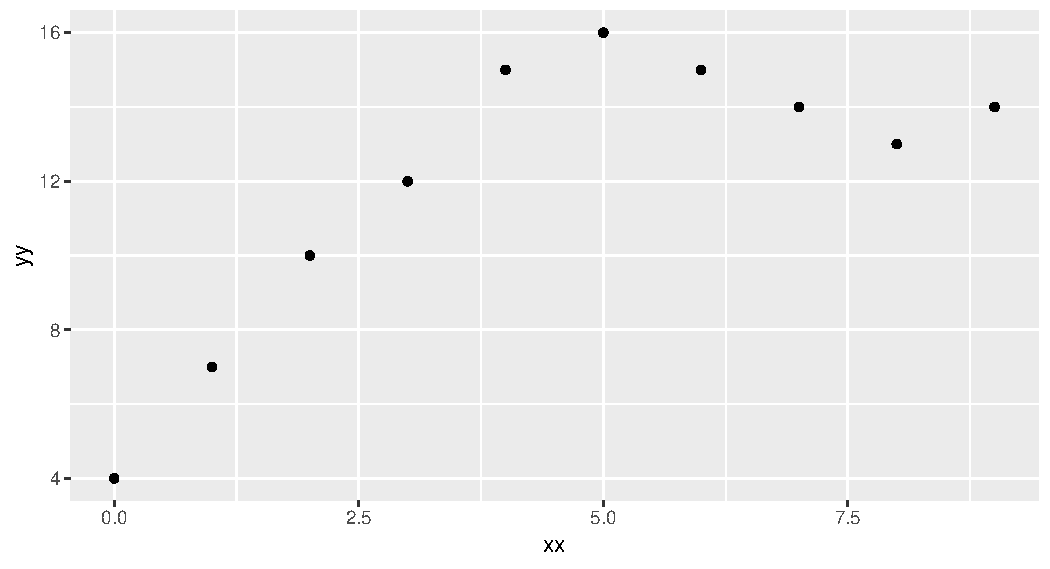
\includegraphics[width=\maxwidth]{figure/unnamed-chunk-18-1} 

\end{knitrout}
  
  
\end{frame}

\begin{frame}[fragile]{Comments on graphs}
  
  \begin{itemize}
  \item For subjects who were at rest, no change in pulse rate over
    time, for both diet groups.
  \item For walking subjects, not much change in pulse rates over
    time. Maybe a small increase on average between 1 and 15 minutes.
  \item For both running groups, an overall increase in pulse rate
    over time, but the increase is stronger for the \texttt{lowfat}
    group.
  \item No consistent effect of diet over all exercise groups.
  \item No consistent effect of exercise type over both diet groups.
  \item No consistent effect of time over all diet-exercise type combos.
  \end{itemize}
  
\end{frame}

\begin{frame}[fragile]{``Simple effects'' of diet for the subjects who ran}
  
  \begin{itemize}
  \item Looks as if there is only any substantial time effect for the
    runners. For them, does diet have an effect?
  \item Pull out only the runners from the wide data:
\begin{knitrout}
\definecolor{shadecolor}{rgb}{0.969, 0.969, 0.969}\color{fgcolor}\begin{kframe}
\begin{alltt}
\hlstd{runners.wide}\hlkwb{=}\hlkwd{filter}\hlstd{(exercise.wide,exertype}\hlopt{==}\hlstr{"running"}\hlstd{)}
\end{alltt}
\end{kframe}
\end{knitrout}
\item Create response variable and do MANOVA. Some of this looks like
  before, but I have different data now:
  
\begin{knitrout}
\definecolor{shadecolor}{rgb}{0.969, 0.969, 0.969}\color{fgcolor}\begin{kframe}
\begin{alltt}
\hlstd{response}\hlkwb{=}\hlkwd{with}\hlstd{(runners.wide,}\hlkwd{cbind}\hlstd{(min01,min15,min30))}
\hlstd{runners.1}\hlkwb{=}\hlkwd{lm}\hlstd{(response}\hlopt{~}\hlstd{diet,}\hlkwc{data}\hlstd{=runners.wide)}
\hlstd{times}\hlkwb{=}\hlkwd{colnames}\hlstd{(response)}
\hlstd{times.df}\hlkwb{=}\hlkwd{data.frame}\hlstd{(times)}
\hlstd{runners.2}\hlkwb{=}\hlstd{car}\hlopt{::}\hlkwd{Manova}\hlstd{(runners.1,}\hlkwc{idata}\hlstd{=times.df,}
                 \hlkwc{idesign}\hlstd{=}\hlopt{~}\hlstd{times)}
\end{alltt}
\end{kframe}
\end{knitrout}
  \end{itemize}
  
\end{frame}

\begin{frame}[fragile]{Results}
  
  {\footnotesize
\begin{knitrout}
\definecolor{shadecolor}{rgb}{0.969, 0.969, 0.969}\color{fgcolor}\begin{kframe}
\begin{alltt}
\hlstd{runners.2}
\end{alltt}
\begin{verbatim}
## 
## Type II Repeated Measures MANOVA Tests: Pillai test statistic
##             Df test stat approx F num Df den Df    Pr(>F)    
## (Intercept)  1   0.99912   9045.3      1      8 1.668e-13 ***
## diet         1   0.84986     45.3      1      8 0.0001482 ***
## times        1   0.92493     43.1      2      7 0.0001159 ***
## diet:times   1   0.68950      7.8      2      7 0.0166807 *  
## ---
## Signif. codes:  0 '***' 0.001 '**' 0.01 '*' 0.05 '.' 0.1 ' ' 1
\end{verbatim}
\end{kframe}
\end{knitrout}
  }
  
  \begin{itemize}
  \item The \texttt{diet} by \texttt{time} interaction is still
    significant (at $\alpha=0.05$): the effect of time on pulse rates is different for
    the two diets.
  \item At $\alpha=0.01$, the interaction is not significant, and then
    we have only two (very) significant main effects of \texttt{diet}
    and \texttt{time}. 
  \end{itemize}
  
\end{frame}

\begin{frame}[fragile]{How is the effect of diet different over time?}
  
  \begin{itemize}
  \item Table of means. Only I need long data for this, so make it (in
    a pipe):
    
\begin{knitrout}
\definecolor{shadecolor}{rgb}{0.969, 0.969, 0.969}\color{fgcolor}\begin{kframe}
\begin{alltt}
\hlstd{runners.wide} \hlopt
  \hlkwd{gather}\hlstd{(time,pulse,min01}\hlopt{:}\hlstd{min30)} \hlopt
  \hlkwd{group_by}\hlstd{(time,diet)} \hlopt
  \hlkwd{summarize}\hlstd{(}\hlkwc{mean}\hlstd{=}\hlkwd{mean}\hlstd{(pulse),} \hlkwc{sd}\hlstd{=}\hlkwd{sd}\hlstd{(pulse))} \hlkwb{->} \hlstd{summ}
\end{alltt}
\end{kframe}
\end{knitrout}

\item Result of \texttt{summarize} is data frame, so can save it (and
  do more with it if needed).

  \end{itemize}
  
\end{frame}

\begin{frame}[fragile]{Understanding diet-time interaction}

  \begin{itemize}
    \item The summary:
\begin{knitrout}
\definecolor{shadecolor}{rgb}{0.969, 0.969, 0.969}\color{fgcolor}\begin{kframe}
\begin{alltt}
\hlstd{summ}
\end{alltt}
\begin{verbatim}
## Source: local data frame [6 x 4]
## Groups: time [?]
## 
##    time      diet  mean        sd
##   <chr>    <fctr> <dbl>     <dbl>
## 1 min01    lowfat  98.2  3.701351
## 2 min01 nonlowfat  94.0  4.527693
## 3 min15    lowfat 124.4  8.619745
## 4 min15 nonlowfat 109.8 13.122500
## 5 min30    lowfat 140.6  7.197222
## 6 min30 nonlowfat 111.4  7.924645
\end{verbatim}
\end{kframe}
\end{knitrout}
  \item Pulse rates at any given time higher for \texttt{lowfat} (diet
  effect), 
  \item Pulse rates increase over time of exercise (time effect),
    
  \item but the \emph{amount by which pulse rate higher} for a diet depends on
  time: \texttt{diet} by \texttt{time} interaction.

  \end{itemize}
  
\end{frame}


\begin{frame}[fragile]{Interaction plot}
\begin{itemize}
\item We went to trouble of finding means by group, so making
  interaction plot is now mainly easy:
  
\begin{knitrout}
\definecolor{shadecolor}{rgb}{0.969, 0.969, 0.969}\color{fgcolor}\begin{kframe}
\begin{alltt}
\hlkwd{ggplot}\hlstd{(summ,}\hlkwd{aes}\hlstd{(}\hlkwc{x}\hlstd{=time,}\hlkwc{y}\hlstd{=mean,}\hlkwc{colour}\hlstd{=diet,}\hlkwc{group}\hlstd{=diet))}\hlopt{+}
  \hlkwd{geom_point}\hlstd{()}\hlopt{+}\hlkwd{geom_line}\hlstd{()}
\end{alltt}
\end{kframe}
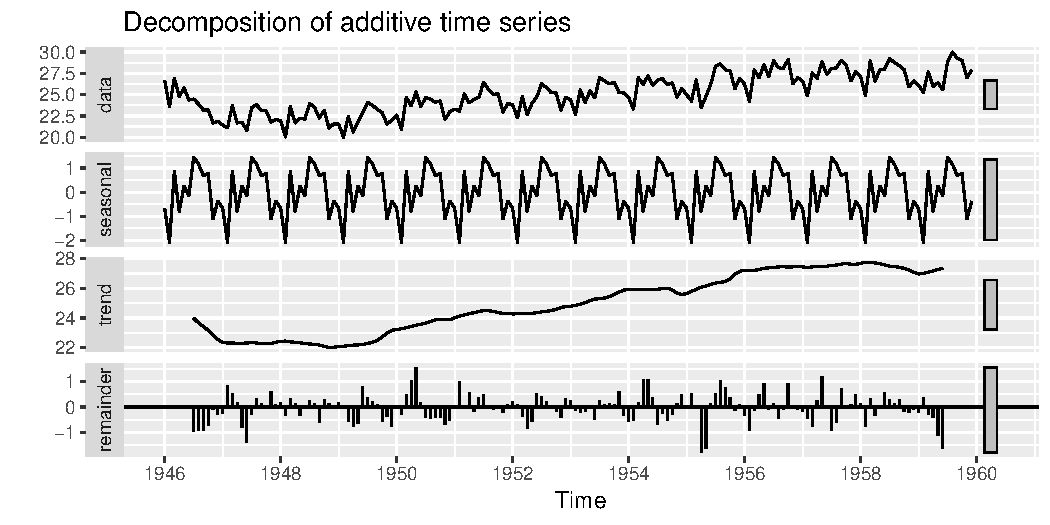
\includegraphics[width=\maxwidth]{figure/unnamed-chunk-24-1} 

\end{knitrout}

\item The lines are not parallel, so there is interaction between diet
  and time.
\end{itemize}
  
\end{frame}
